\documentclass[12pt]{article}
\usepackage[T1]{fontenc}
\usepackage[polish]{babel}
\usepackage[utf8]{inputenc}
\usepackage{graphicx}
\usepackage{amsmath}

\graphicspath{ {./images} }

\begin{document}

\title{{\Large}Zadanie numeryczne 9}
\date{}
\author{Jakub Heczko}

\maketitle

\section{Wprowadzenie do problemu: }
Problemem zadania było rozwiązanie równiania charakterystycznego pewnej macierzy. Zadanie sprowadzało, się do znalezienia miejsc zerowych naszej funkcji
\section{Uproszczenie problemu: }
Zacznijmy może od tego jak wygląda nasza macierz:
\[
\begin{bmatrix}
    4 & -1 & 0 \\
    -1 & 4 & -1 \\ 
    0 & -1 & 4 \\
\end{bmatrix}
\]
Nastepnie po zapisaniu i uproszczeniu wyznacznika dostajemy funkcję następującej postaci:
\begin{center}
    \begin{math}
        f(x) = -x^{3}+12x^{2}-46x+56
    \end{math}
\end{center}
Taka funkcja wygląda następująco na wykresie:
\newline
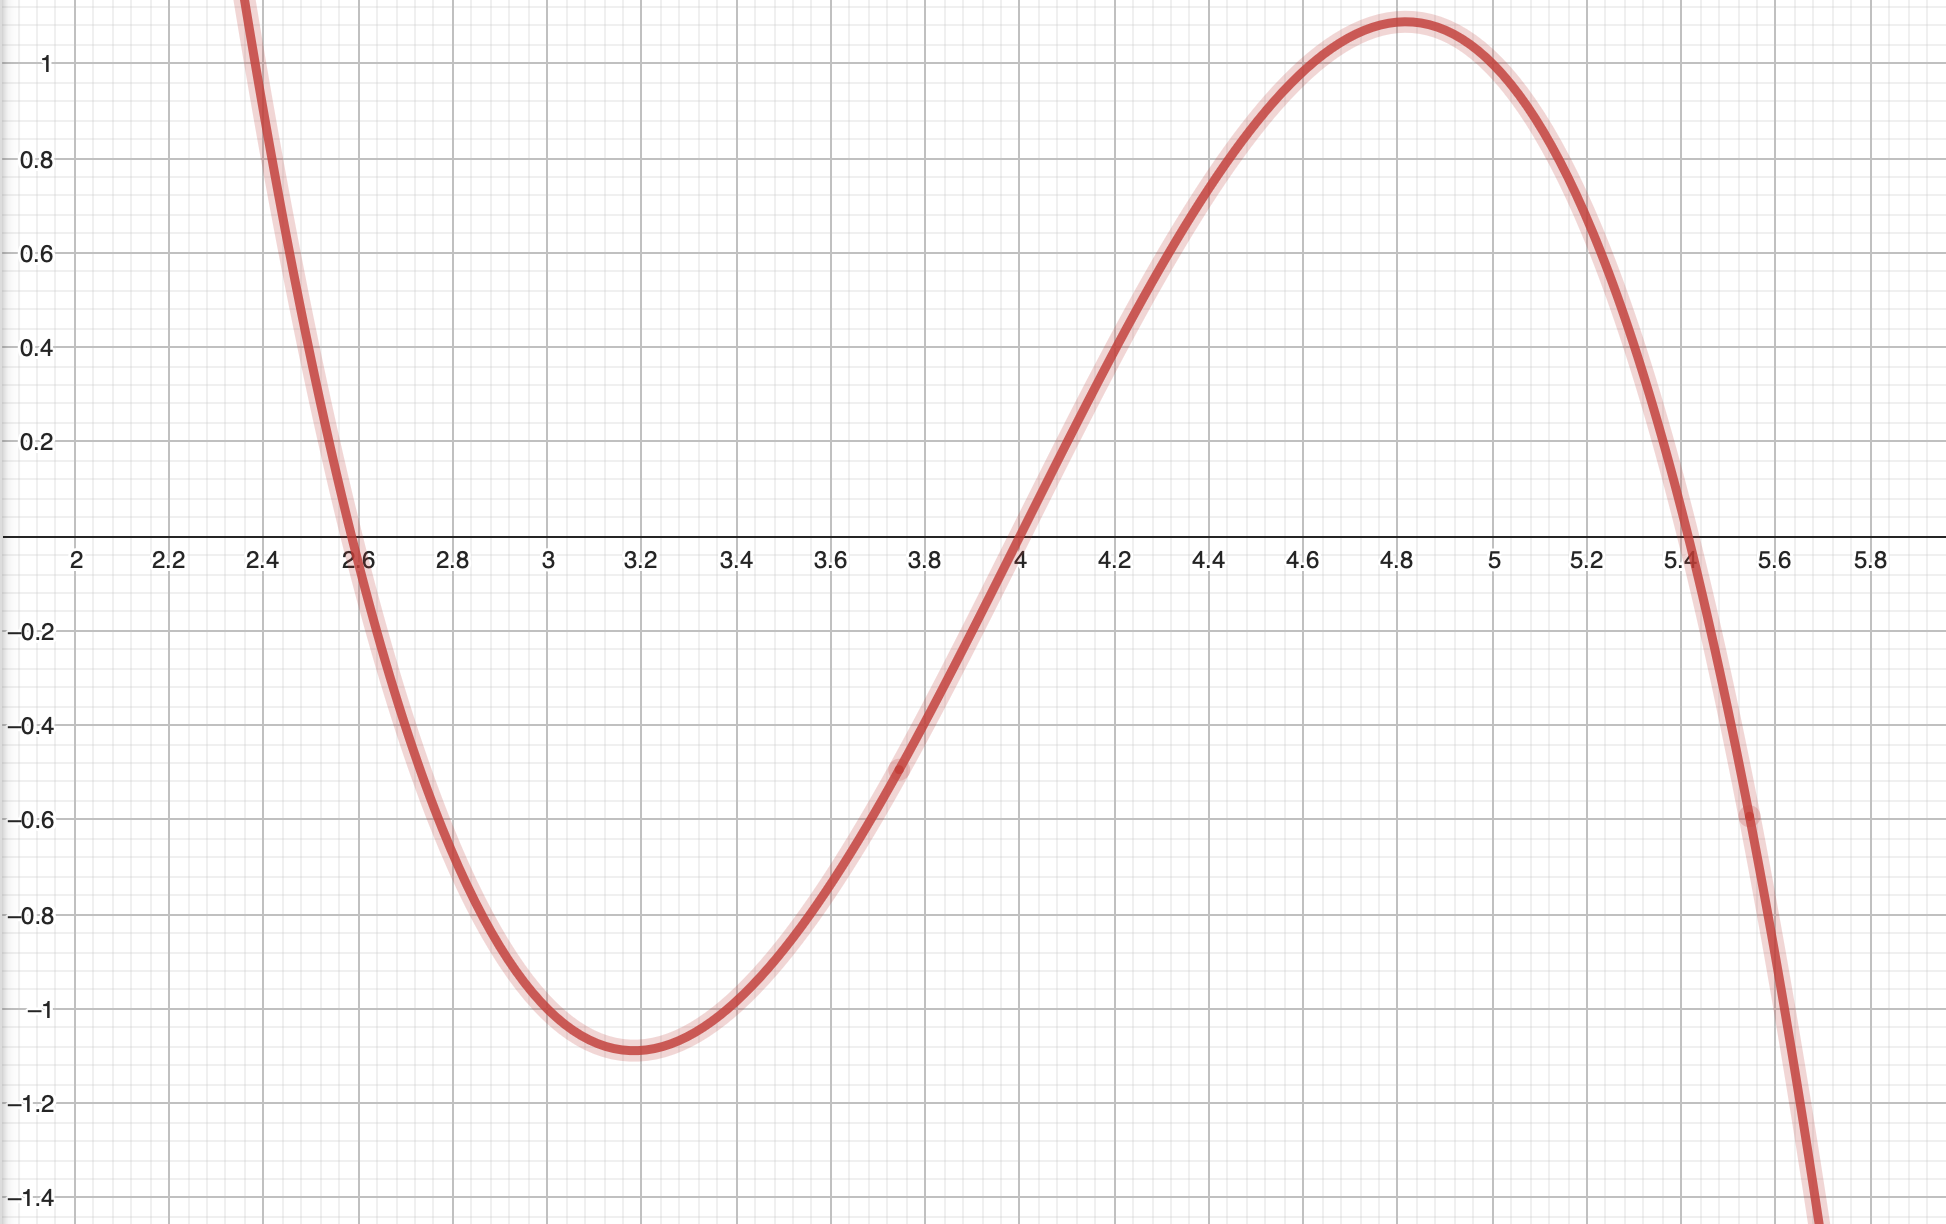
\includegraphics[width=12cm,height=8cm, keepaspectratio]{wykres_funkcja.png}
\newline
Jak widzimy osiąga ona miejsca zerowe w $x_{1} = -2,585786437626905$ oraz $x_{2} = 4$ oraz $x_{3} = 5,414213562373095$
\newline
Teraz, aby znaleźć nasze miejsca zerowe, użyje trzech funkcji, które każde z nich po kolei omówie, pierwszą będzie metodą bisekcji, nastepną metoda regula falsi i na samym końcu metoda siecznych. 
\subsection{Metoda Bisekcji:}
\subsection{Metoda Regula Falsi:}
\subsection{Metoda Siecznych:}
\section{Wyniki:}
Bisekcja iteracje:  52\newline
Bisekcja: [2.5857864394783974, 4.0, 5.414213560521603]\newline
Falsi iteracje:  40\newline
Falsi:  [2.5857864434036886, 4.0, 6]\newline
Sieczne iteracje:  15\newline
Siecznych:  [2.5857864376268997, 4.0, 5.414213562373092]\newline
Jak widać najszybciej z nich wszystkich poradziła sobie metoda siecznych, która praktycznie trzy-krotnie skróciła naszą ilośc iteracji
\end{document}